% ============================================================
% C2 Challenge: AI for Math  --  paper.tex
% From Natural Language to Verifiable Reasoning:
% A Semantic Reduction Framework for Reliable AI Mathematics
%
% 编译：pdflatex paper.tex && bibtex paper && pdflatex paper.tex && pdflatex paper.tex
% 要求：可独立编译，引用可解析。references.bib 中 11 篇全部经人工核验。
% ============================================================

\documentclass[11pt,a4paper]{article}

\usepackage[utf8]{inputenc}
\usepackage[T1]{fontenc}
\usepackage[margin=1in]{geometry}
\usepackage{amsmath,amssymb}
\usepackage{graphicx}
\usepackage{booktabs}
\usepackage{tikz}
\usepackage{hyperref}

\usetikzlibrary{positioning}

\title{From Natural Language to Verifiable Reasoning:\\
A Semantic Reduction Framework for Reliable AI Mathematics}

\author{Feng Shuo}

\date{\today}

\begin{document}
\maketitle

% ------------------------------------------------------------
\begin{abstract}
Large language models produce mathematical arguments that are fluent but not
trustworthy: a proof may read correctly and still be wrong.  We argue that this
failure is not primarily a failure of generation, nor of verification, but of
the \emph{middle layer} that connects them.  We decompose an AI4Math system into
three layers --- generation, semantic reduction, and verification --- and show
that the second layer is the actual bottleneck: verification can only operate on
computable objects, and natural language is not one.  We then make the argument
operational in two ways.  First, we give a taxonomy of four reduction failure
classes, each with a machine-checkable detection criterion, showing that all
four are invisible to a stronger prover.  Second, we introduce
\emph{certified accuracy} as a metric distinct from reported accuracy, and prove
an identity that decomposes the latter into an auditable part and an unauditable
part.  The practical consequence is that a system can improve its reported
accuracy while becoming \emph{less} verifiable, and that current benchmarks
cannot detect this.  We corroborate the bottleneck claim in two independent ways.  Published
end-to-end evidence composes a $97\%$-accurate autoformaliser with a
$69\%$-accurate prover and obtains roughly $36\%$ end-to-end accuracy, the loss
being traced to formal--informal mismatch.  And we report a first measurement of
our own: across GSM8K and two MATH subjects, one model's reported accuracy falls
by less than five points ($0.980 \to 0.933$) while the share of its own correct
answers that survives machine audit falls from $0.67$ to $0.12$.  The failures
concentrate in the reduction layer and none of them is visible to a stronger
verifier.  We also find that $\nu$ is not stable across runs of a fixed hosted
model, moving by up to $16$ points, which is itself an argument for measuring it
rather than assuming it.  We do not claim a new solver; we claim a sharper
decomposition, a testable taxonomy, and a measurable target.

\noindent\textbf{Keywords:} AI for mathematics, formal verification, semantic
reduction, neuro-symbolic systems, reliability, evaluation methodology
\end{abstract}

% ------------------------------------------------------------
\section{Introduction}

Machine learning has entered core mathematical practice.  Neural models guided
human intuition toward new results in knot theory and representation
theory~\cite{davies2021advancing}; an evolutionary procedure paired with a
program evaluator discovered new cap-set constructions beyond the best known
ones~\cite{romera2024funsearch}; and a neuro-symbolic system solved 25 of 30
olympiad geometry problems~\cite{trinh2024alphageometry}.

Yet these successes sit next to an uncomfortable observation.  Language models
regularly emit reasoning chains that are locally plausible and globally
wrong~\cite{wei2022chain}.  On competition-level benchmarks such as
MATH~\cite{hendrycks2021math} and GSM8K~\cite{cobbe2021gsm8k}, a correct final
answer does not certify a correct derivation.  Process supervision, which labels
intermediate steps rather than only outcomes, improves
reliability~\cite{lightman2023lets} --- but it is expensive precisely because
there is no machine-checkable handle on an intermediate step written in natural
language.

The field's dominant response has been to add verification on top of generation.
We contend that this response is aimed one layer too high.  Verification
instruments operate on objects that already possess a decidable notion of
well-formedness; a natural-language derivation possesses none.  Something must
therefore stand between the two, and that something is where we claim the
failures concentrate.

\paragraph{Claim.}
Reliability cannot be bought by final-answer verification alone.  It requires an
explicit \emph{semantic reduction layer} that maps natural-language reasoning
into a structured object a verifier can act on --- and that layer must be
measured, not assumed.

\paragraph{Contributions.}
\begin{enumerate}
  \item A three-layer decomposition of AI4Math systems that isolates semantic
        reduction as a first-class component rather than as preprocessing.
  \item A structural argument, plus a decomposition identity
        (Section~\ref{sec:bottleneck}), showing that most observed failures
        concentrate in that layer.
  \item A taxonomy of four reduction failure classes, each paired with a
        machine-checkable detection criterion (Section~\ref{sec:taxonomy}).
  \item \emph{Certified accuracy} as a metric distinct from reported accuracy, a
        reliability checklist, and an evaluation protocol that reports both
        (Sections~\ref{sec:framework} and~\ref{sec:protocol}).
\end{enumerate}

We are explicit about scope: this paper proposes no new solver.  It is analytic
in its main contribution --- a sharper decomposition and metrics that make the
central claim falsifiable --- but Section~\ref{sec:protocol} does report
measurements, on one hosted model and three school-level corpora, and
Section~\ref{sec:protocol-sens} is explicit about how much of what we measured
belongs to our apparatus rather than to the model.

% ------------------------------------------------------------
\section{A Three-Layer Decomposition}
\label{sec:decomp}

Let an AI4Math system be decomposed as
\begin{equation}
  G \;\longrightarrow\; R \;\longrightarrow\; V,
  \label{eq:pipeline}
\end{equation}
where $G$ is generation, $R$ is semantic reduction, and $V$ is verification.
Figure~\ref{fig:pipeline} places the three layers in their usual pipeline
setting, where natural language serves as the \emph{interface} at both ends and
the reduced object is the \emph{kernel} in the middle.

\begin{figure}[t]
\centering
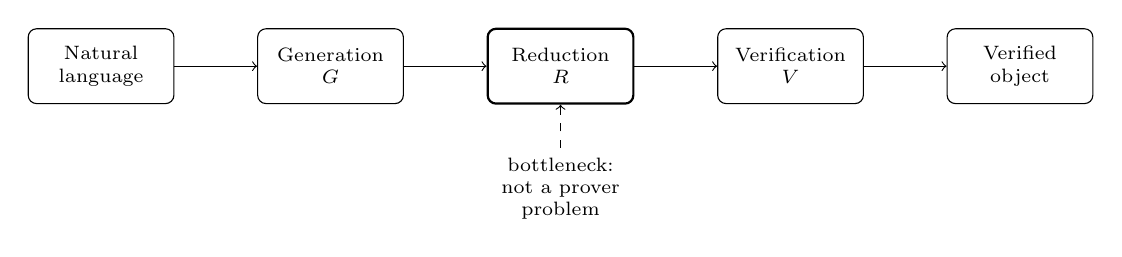
\begin{tikzpicture}[
  node distance=1.05cm,
  box/.style={rectangle, draw, rounded corners=3pt, minimum height=0.95cm,
              minimum width=1.85cm, align=center, font=\scriptsize},
  crit/.style={rectangle, draw, rounded corners=3pt, minimum height=0.95cm,
               minimum width=1.85cm, align=center, font=\scriptsize,
               line width=0.8pt}
]
\node[box] (nl)  {Natural\\language};
\node[box, right=of nl] (g) {Generation\\$G$};
\node[crit, right=of g] (r) {Reduction\\$R$};
\node[box, right=of r] (v) {Verification\\$V$};
\node[box, right=of v] (ob) {Verified\\object};
\draw[->] (nl) -- (g);
\draw[->] (g) -- (r);
\draw[->] (r) -- (v);
\draw[->] (v) -- (ob);
\node[below=0.55cm of r, font=\scriptsize, align=center, text width=2.6cm] (note)
  {bottleneck:\\not a prover\\problem};
\draw[->, dashed] (note) -- (r);
\end{tikzpicture}
\caption{The three-layer decomposition of an AI4Math system.  Natural language
is the interface; the reduced object is the kernel.  Our claim is that failures
concentrate in $R$, and that strengthening $V$ cannot compensate.}
\label{fig:pipeline}
\end{figure}

\subsection{Layer 1: Generation}
A language model emits a natural-language reasoning chain, typically via
chain-of-thought prompting~\cite{wei2022chain}.  Its output is probabilistic,
untyped, and semantically underspecified.  Nothing in this layer offers a handle
by which a machine could reject a step.

\subsection{Layer 2: Semantic Reduction}
Natural language is mapped to a structured representation: first- or
higher-order logic expressions, executable programs, proof objects, or a typed
intermediate representation.  The theoretical anchor is the
Curry--Howard correspondence, under which a proof is a program and a formula is
a type.  The output of this layer is the \emph{only} thing Layer~3 will ever
see.

\subsection{Layer 3: Verification}
A formal system checks self-consistency, derivability, factual grounding, or
constraint satisfaction.  In practice this is an interactive theorem prover such
as Lean~4~\cite{moura2021lean4} over the mathlib
library~\cite{mathlib2020}, or a symbolic/SMT solver.  The cross-system
benchmark miniF2F~\cite{zheng2022minif2f} shows that this layer is now
measurable and comparable across provers.

A useful contrast is physics-informed neural
networks~\cite{raissi2019pinn}, where the ``verifier'' is not a proof kernel but
a continuous residual: the network is penalized for violating a differential
equation.  This shows that $V$ need not be symbolic, but it does not change the
requirement that whatever $V$ consumes must already be a formal object.  The
residual is computable precisely because the PDE was written down formally in
advance.

% ------------------------------------------------------------
\section{The Semantic Reduction Bottleneck}
\label{sec:bottleneck}

We claim that when an AI4Math system fails, it fails in Layer~2 more often than
in Layers~1 or~3.

\subsection{The structural argument}
Verification is only defined over objects with a decidable notion of
well-formedness.  Natural language has none.  Therefore, if Layer~2 produces no
object, or produces an object that does not faithfully encode the intended
claim, then Layer~3 has nothing to check --- or checks the wrong thing.  Two
consequences follow.

\begin{enumerate}
  \item \textbf{Verification failure masquerading as reasoning failure.}  The
        pipeline reports ``unverified'' rather than ``unreduced'', conflating a
        translation failure with a mathematical one.  The diagnostic signal is
        destroyed at the point where it would be cheapest to act on.
  \item \textbf{Undetectable hallucination.}  An unfaithful translation can be
        internally consistent and still prove a proposition different from the
        one that was asked.  A sound kernel certifies the object it was given,
        not the intention behind it.
\end{enumerate}

This reframes the reliability problem: the scarce resource is not the prover's
power but the \emph{fidelity of the translation}.

\subsection{A decomposition identity}
\label{sec:identity}

The argument becomes testable once written as an identity.  Fix a benchmark of
$N$ problems.  Let $V \subseteq \{1,\dots,N\}$ be the subset for which
reduction yields a well-formed, machine-checkable object, and let
$\nu = |V|/N$ be the \emph{verifiability rate}.  Let $a$ be reported
final-answer accuracy, let
\begin{equation}
  \alpha \;=\; \frac{1}{N}\,
  \bigl|\{\,i \in V : \text{object verified and consistent with intent}\,\}\bigr|
  \label{eq:certified}
\end{equation}
be \emph{certified accuracy}, and let $u$ be the accuracy on the complement
$V^{c}$ --- correct final answers that carry no machine-checkable warrant.  Then
\begin{equation}
  a \;=\; \alpha \;+\; (1-\nu)\,u,
  \qquad\text{and}\qquad \alpha \;\le\; a .
  \label{eq:decomp}
\end{equation}

Equation~(\ref{eq:decomp}) is an accounting identity, not a model, and its
content is entirely in the second term.  The quantity $(1-\nu)u$ is exactly the
part of reported accuracy that cannot be audited.  A system may therefore
\emph{increase} $a$ while \emph{decreasing} $\nu$: it can become better at
producing answers and worse at producing reasons that can be checked, and a
benchmark reporting only $a$ will record this as progress.  No benchmark we are
aware of reports $\nu$, so no current leaderboard can detect this regression.
This is the concrete sense in which the field is measuring the wrong quantity.

\subsection{Empirical support}
\label{sec:evidence}

The argument above is structural.  It is corroborated by a recent end-to-end
evaluation that measures exactly the quantity we claim is unmeasured.  Ospanov,
Farnia, and Yousefzadeh~\cite{ospanov2025minif2f} place a model in an
``olympiad setting'': read the informal statement, formalise it in Lean, prove
it, and receive credit only if the proved statement corresponds to the original
informal one.  Under this protocol, the best pipeline accuracy is about
$36\%$, against component-level accuracies of $97\%$ reported for
autoformalisation and $69\%$ for theorem proving.  The composition of two
strong components yields far less than either.  Analysing the failure modes,
the authors trace a considerable portion of the drop to discrepancies between
formal and informal statements affecting more than half of miniF2F's problems,
and report that only $59\%$ of the formal statements in the test split are
correct.

Two readings are possible, and both support our thesis.  Under the first, the
loss occurs because the formal statements were written carelessly --- a
benchmark-quality failure.  Under the second, it occurs because the
autoformaliser and the prover optimise different objectives --- a
Layer~2 fidelity failure.  These are not competing explanations; a benchmark
that does not police Layer~2 cannot detect either.  Note also that the authors'
corrected benchmark raises end-to-end accuracy substantially, which shows that
the loss was never in the prover.  We therefore treat this result as evidence
that Equation~(\ref{eq:decomp})'s unauditable term is not a small correction but
potentially the dominant one.

% ------------------------------------------------------------
\section{Analysis: A Taxonomy of Reduction Failures}
\label{sec:taxonomy}

The bottleneck claim is only useful if reduction failures can be told apart.
We propose four classes, distinguished by \emph{where in the pipeline they
become detectable}.  The taxonomy is deliberately syntactic: each class is
paired with a criterion a system can evaluate without human judgement, so that
the classes are reportable rather than merely descriptive.

Table~\ref{tab:taxonomy} states the four classes with their criteria.

\begin{table}[t]
\centering
\caption{Four classes of semantic reduction failure.  The rightmost column is
the point of the framework: no class is recoverable by strengthening the
verifier.}
\label{tab:taxonomy}
\small
\begin{tabular}{@{}lp{5.0cm}p{4.6cm}p{2.1cm}@{}}
\toprule
Class & Failure & Detection criterion & Visible to $V$? \\
\midrule
A & \emph{Ambiguity}: one surface form admits several well-typed formal readings
  & Parse multiplicity $>1$ under the target type system & No --- $V$ receives one parse \\
\addlinespace
T & \emph{Type omission}: implicit domain, coercion, or side condition silently dropped
  & Elaboration leaves unresolved metavariables or inserts defaults & No --- $V$ sees a well-typed term \\
\addlinespace
R & \emph{Referential drift}: anaphora or scope binds to a wrong antecedent across steps
  & IR graph retains unresolved or multi-candidate coreference edges & No --- $V$ checks the resulting graph \\
\addlinespace
N & \emph{Non-invertibility}: the verified proposition differs from the intended one
  & Round-trip mismatch between $\mathrm{render}(\mathrm{parse}(x))$ and $x$ & No --- $V$ proves what it was given \\
\bottomrule
\end{tabular}
\end{table}

\paragraph{Why the taxonomy matters.}
Classes A, T, and R are all \emph{pre-verification} failures: by the time an
object reaches $V$, the error has already been compiled into it, and a sound
kernel will faithfully certify the wrong claim.  Class~N is the inverse failure
and is the most damaging, because it is invisible in both directions: the proof
is valid and the rendering reads correctly, yet the two no longer correspond.
None of the four is mitigated by a stronger prover, a larger model, or more
search --- which is precisely the sense in which Layer~2 is a bottleneck rather
than a weak link that better neighbours can compensate for.

\paragraph{Relation to existing error analyses.}
Prior work on process supervision~\cite{lightman2023lets} labels erroneous steps
but does not classify \emph{why} a step cannot be checked; our taxonomy is
orthogonal to, and composable with, such labels.  A step can be judged correct
by a human labeler and still fall into class~T, because the omission is
invisible in natural language.

% ------------------------------------------------------------
\section{Proposed Framework}
\label{sec:framework}

\subsection{Typed intermediate representation}
\label{sec:ir}
We propose a typed IR with four components: a type system, an operational
semantics, a constraint system, and a composable graph/AST structure.  The IR is
not a new logic; it is the interface contract that makes Layers~1 and~3
separately auditable.  We sketch it as a small explicitly typed term language
with types $\tau$, terms $e$, and propositions $\phi$:
\[
\begin{array}{rcl}
\tau & ::= & \mathbb{N} \mid \mathbb{Z} \mid \mathbb{Q} \mid \mathbb{R}
            \mid \tau \to \tau \mid \mathrm{Set}(\tau) \\[2pt]
e & ::= & x \mid n \mid e + e \mid e \times e \mid e/e
          \mid \mathrm{apply}(e,e) \mid \mathbf{let}\;x:\tau = e\;\mathbf{in}\;e \\[2pt]
\phi & ::= & e \le e \mid e = e \mid \phi \land \phi \mid \phi \Rightarrow \phi
            \mid \forall x{:}\tau.\,\phi
\end{array}
\]
with the side condition that every division carries an explicit non-zero proof
obligation.  That obligation is exactly the one whose silent discharge
constitutes class~T of Section~\ref{sec:taxonomy}.  A term counts as
well-formed only if elaboration discharges every such obligation; a reduction
that leaves any obligation unresolved is reported as \emph{unreduced}, never as
verified.

\subsection{Bidirectional consistency}
We require $\mathrm{IR} \leftrightarrow \text{natural language}$ to be both
interpretable and traceable: every IR node records the span it came from, and
every rendered sentence records the node it came from.  This property is what
makes human audit possible, and it is the mechanism that exposes class~N
failures through round-tripping.

\subsection{A reliability checklist}
\label{sec:checklist}
The framework is only as good as its enforcement.  We state five requirements
as a checklist, each traceable to a failure class above.

\begin{enumerate}
  \item \textbf{Provenance.}  Every IR node carries the source span it was
        reduced from.  (Enables audit; exposes class~R.)
  \item \textbf{Explicit elaboration.}  Implicit domains, coercions, and side
        conditions are elaborated or flagged.  Silent defaults are prohibited.
        (Exposes class~T.)
  \item \textbf{Parse determinism.}  A reduction with multiplicity $>1$ is
        reported as ambiguous, not resolved by sampling.  (Exposes class~A.)
  \item \textbf{Round-trip audit.}  $\mathrm{render}(\mathrm{parse}(x))$ is
        compared against $x$; mismatches are reported, never repaired silently.
        (Exposes class~N.)
  \item \textbf{Reject, do not repair.}  A failed reduction reports
        ``unreduced''.  It must never be reported as ``verified'' or silently
        downgraded to an unchecked answer.
\end{enumerate}

Requirement~5 is the one most likely to be violated in practice, because it
lowers reported accuracy.  We regard that as the point: the checklist trades
apparent performance for auditable performance.

% ------------------------------------------------------------
\section{Evaluation Protocol}
\label{sec:protocol}

\subsection{Benchmarks}
\label{sec:protocol-benchmarks}
GSM8K~\cite{cobbe2021gsm8k} and MATH~\cite{hendrycks2021math} for informal
reasoning; miniF2F~\cite{zheng2022minif2f} for formal proving.  We note a
methodological caveat discussed in Section~\ref{sec:rw-verify}: miniF2F
statements are human-formalized, so it exercises Layer~3 but not Layer~2.

Two filters are applied to every task and must be stated because they shape the
numbers.  First, only problems whose reference answer is an integer are scored.
This is a grading decision, not a modelling one: a reference of $1/11$ is stored
as $0.09090909090909091$, so a model that correctly writes $0.0909$ is off by
$9.1\times10^{-6}$ and would be marked wrong for writing fewer digits.
Restricting to integers makes ``correct'' a fact about the answer rather than
about its decimal rendering.  It removes $14.1\%$ of MATH prealgebra and $8.3\%$
of number theory.  Second, we take the first 200 surviving problems of each test
split rather than sampling, so the subset is reproducible without a seed.

\subsection{Metrics}
Table~\ref{tab:metrics} defines the reported quantities.  The protocol's only
hard requirement is that $a$ is never reported alone.

\begin{table}[t]
\centering
\caption{Reported metrics.  $\nu$, $\kappa$, and $\alpha$ are defined only over
outputs that reach Layer~3; $a$ is defined over all outputs.}
\label{tab:metrics}
\begin{tabular}{@{}clp{5.4cm}@{}}
\toprule
Symbol & Name & Definition \\
\midrule
$a$ & Accuracy & Fraction of final answers matching the reference \\
$\nu$ & Verifiability rate & Fraction of outputs for which $R$ yields a well-formed object \\
$\kappa$ & Consistency & Fraction of verified objects whose rendering matches the intended claim \\
$\alpha$ & Certified accuracy & Fraction of \emph{all} outputs that are verifiable, verified, consistent, \emph{and correct} \\
\bottomrule
\end{tabular}
\end{table}

\subsection{Comparison}
A pure LLM baseline against an IR-based pipeline, with $\nu$ and $\alpha$
reported for both.  The prediction implied by
Section~\ref{sec:bottleneck} is falsifiable: the IR pipeline should show lower
$a$ but strictly positive $\nu$ and $\alpha$, whereas the baseline should show
$\nu = \alpha = 0$ regardless of $a$.

\subsection{An illustrative calculation}
The identity can also be exercised on figures published elsewhere.  We label
this an illustration, not one of our measurements.  Using
the component accuracies reported for the miniF2F
pipeline~\cite{ospanov2025minif2f} --- $97\%$ for autoformalisation and $69\%$
for theorem proving --- a naive composition under an independence assumption
gives $0.97 \times 0.69 \approx 0.67$.  The same work reports end-to-end
accuracy of about $0.36$ under the stricter criterion that credit requires the
proved statement to correspond to the original informal one.  Read through
Equation~(\ref{eq:decomp}), the unauditable term is therefore of order
$0.67 - 0.36 \approx 0.31$: roughly thirty points of nominally reported accuracy
carry no machine-checkable warrant.

Two caveats are binding.  The independence assumption is ours and is not
defended by that work; and the correspondence criterion behind $0.36$ is
stricter than the one implicit in $0.67$, so the two quantities are not strictly
like-for-like.  We offer the calculation as an order-of-magnitude indication.

\subsection{Results}
Table~\ref{tab:results} fills in the reporting form with measured values.  Its
hard requirement is unchanged: no cell may be inferred from another, so $\alpha$
is counted rather than derived from $a$ and $\nu$.

\begin{table}[t]
\centering
\caption{Measured results on three task distributions, one model
(\texttt{deepseek-v4-flash}, temperature~0), one harness, one session.  The
baseline column is free-form chain-of-thought; the IR columns are the same model
asked to emit the typed IR of Section~\ref{sec:framework}.  $\kappa$ is
conditioned on outputs that parse and evaluate; $\alpha$ is over all outputs.
$n < 200$ for the MATH rows because problems with a non-integer reference answer
are excluded (Section~\ref{sec:protocol-benchmarks}).}
\label{tab:results}
\begin{tabular}{@{}lcccccc@{}}
\toprule
Task & $n$ & baseline $a$ & IR $a$ & $\nu$ & $\kappa$ & $\alpha$ \\
\midrule
GSM8K                    & 200 & 0.980 & 0.680 & 0.835 & 0.825 & 0.660 \\
MATH, prealgebra         & 170 & 0.959 & 0.500 & 0.618 & 0.848 & 0.435 \\
MATH, number theory      & 195 & 0.933 & 0.349 & 0.626 & 0.592 & 0.113 \\
\bottomrule
\end{tabular}
\end{table}

\paragraph{Reading the table.}
The baseline column is nearly flat: $0.980$, $0.959$, $0.933$.  Read on its own
it says that the model is a competent solver on all three distributions and only
slightly worse on the harder ones.  The $\alpha$ column describes the same model
on the same problems and says something else: $0.660$, $0.435$, $0.113$.
Reported accuracy falls by $4.7$ points across the three rows; certified accuracy
falls by $55$.  Nothing in the first column would let a reader anticipate the
third.

\paragraph{Paired analysis.}
A low $\nu$ admits two explanations that $\nu$ alone cannot separate: the problem
is genuinely hard, or the model can solve it but cannot express the solution in a
checkable form.  Table~\ref{tab:paired} removes the first explanation by
restricting every quantity to the subset of problems the \emph{baseline}
answered correctly.  On that subset the model demonstrably knows the answer, so
whatever the IR condition fails to produce is not a failure to find one.

\begin{table}[t]
\centering
\caption{Paired results, restricted to the problems the baseline solved
(``$s$'').  Task difficulty is controlled by construction: every problem in this
subset was answered correctly by free-form decoding.}
\label{tab:paired}
\begin{tabular}{@{}lcccc@{}}
\toprule
Task & solved & $\nu \mid s$ & $a_{\mathrm{IR}} \mid s$ & $\alpha \mid s$ \\
\midrule
GSM8K               & 196 & 0.837 & 0.689 & 0.668 \\
MATH, prealgebra    & 163 & 0.632 & 0.521 & 0.454 \\
MATH, number theory & 182 & 0.626 & 0.363 & 0.121 \\
\bottomrule
\end{tabular}
\end{table}

This is the paper's central measurement.  Of the answers the model can produce,
the share that survives machine audit falls from two thirds on grade-school
arithmetic to one eighth on number theory, while the share it gets right in the
first place falls by less than five points.  The two quantities describe the same
model on the same problems and they move in opposite directions.

\paragraph{Where the failures land.}
Table~\ref{tab:classes} splits the failures into the classes of
Section~\ref{sec:taxonomy}, separating two things that are easy to conflate:
outputs that never became a checkable object, which is what lowers $\nu$; and
outputs that parsed but then failed to evaluate or whose goal disagreed with
their own stated answer, which is class~N and does not lower $\nu$.

\begin{table}[t]
\centering
\caption{Failure classes.  ``contract'' counts class~T rejections for omitting
the non-zero proof required on division; ``out of grammar'' counts class~R
rejections naming an operation the IR cannot express ($\gcd$, $\bmod$,
$\lfloor\cdot\rfloor$, $\sqrt{\cdot}$).  Both are partly artefacts of our IR
rather than semantic failures, and Section~\ref{sec:protocol-sens} prices them.}
\label{tab:classes}
\small
\begin{tabular}{@{}lcccc@{}}
\toprule
Task & parse-fail & contract (T) & grammar (R) & post-parse (N) \\
\midrule
GSM8K               & 33/200 & 26 &  3 & 30 \\
MATH, prealgebra    & 65/170 & 24 & 27 & 21 \\
MATH, number theory & 73/195 & 19 & 26 & 77 \\
\bottomrule
\end{tabular}
\end{table}

The informative entry is the last column.  These are outputs the checker
accepted as well-formed and then evaluated to a value different from the number
the model itself reported --- the model asserts one thing and its own structured
derivation asserts another.  On GSM8K and prealgebra this happens to about one
output in seven; on number theory, to two in five.  The failures concentrate
exactly where Section~\ref{sec:taxonomy} predicts, in the mapping rather than in
search: no output in any condition failed because a proof could not be found.

\subsection{How much of the failure is our IR's fault?}
\label{sec:sensitivity}
\label{sec:protocol-sens}
Two entries of Table~\ref{tab:classes} are artefacts rather than findings, and
we price them instead of reporting them as reduction failures.

The ``contract'' column counts outputs rejected because a division lacked the
non-zero proof the schema demands.  The rule is ours; a model that ignores it has
failed to follow a contract, not necessarily to preserve meaning.  Waiving it
raises $\nu$ from $0.835$ to $0.965$ on GSM8K, from $0.618$ to $0.759$ on
prealgebra, and from $0.626$ to $0.723$ on number theory.  The gap between
GSM8K and MATH survives the waiver almost unchanged, so the finding does not
depend on that rule.

The ``out of grammar'' column is a stricter objection.  Our IR expresses
arithmetic over rationals and nothing else, so a problem needing $\gcd$, modular
arithmetic, or a floor cannot be expressed in it at all; rejecting such an output
measures our grammar, not the model.  These are $1.5\%$ of GSM8K, $15.9\%$ of
prealgebra and $13.3\%$ of number theory.  We report this rather than filtering
it away, because a reduction layer that cannot carry the semantics of its domain
is a real limitation of the layer --- but the honest reading is that part of the
MATH deficit belongs to the IR design and not to the model.

What remains after both are set aside is the post-parse column, and it is the one
that grows.

\subsection{Reproducibility}
\label{sec:protocol-repro}
$\nu$ turned out to be less stable than we expected, and the instability is a
result rather than a nuisance.  Across repeated runs of the identical
configuration on GSM8K --- same 200 problems, same model string, same
temperature, same harness --- we measured $\nu = 0.995$, $0.835$, $0.800$,
$0.810$ and $0.840$.  The first of these was taken about forty minutes before the
others; the four later runs agree with each other to within $0.04$ and disagree
with the first by $0.16$.  We did not change the prompt, the corpus, or the
checker in between, and a control run with the original phrasing restored gave
$0.840$, so the drift is not attributable to our prompt edit.  Repeated runs on
the MATH subsets are tighter: $\nu = 0.641, 0.618, 0.647$ on prealgebra and
$0.579, 0.626, 0.600$ on number theory.

Two consequences follow.  First, a single $\nu$ measured against a hosted model
should not be read as a property of that model; the ranges above are disjoint
between GSM8K ($0.80$--$0.84$, excluding the drifted first run) and MATH
($0.58$--$0.65$), which is why we claim a task effect at all, but any individual
number carries an uncertainty of a few points that we cannot attribute to a
cause.  Second, and more to the point of this paper: a quantity that moves
$16$ points under a fixed model version is exactly the kind of quantity that
must be reported rather than assumed, and it is not reported today.

\paragraph{Falsification criteria.}
We state in advance what would refute the bottleneck hypothesis, so that the
claim is testable rather than merely plausible:
\begin{itemize}
  \item If $\nu \approx 1$ and $\alpha \approx a$ for a system that performs no
        explicit reduction, then reduction is not a bottleneck and the
        decomposition adds nothing.
  \item If observed failures do not concentrate in classes A--N but appear
        instead as ordinary proof-search failures, the taxonomy is not carving
        at the joint.
  \item If enforcing the checklist raises reported accuracy $a$, then our claim
        that auditable performance trades against apparent performance is wrong.
\end{itemize}

\paragraph{Execution status.}
The numbers in Tables~\ref{tab:results}--\ref{tab:classes} are measured, not
illustrative.  One hosted model (\texttt{deepseek-v4-flash}) at temperature~0
produced every completion behind them --- 1,130 for the three tasks of
Table~\ref{tab:results} (565 problems $\times$ 2 conditions) and 4,090 in total
across the eleven runs of Section~\ref{sec:protocol-repro} --- with no call
failures.  The harness, the corpora, and the verbatim model outputs are
distributed with this paper, so every $\nu$ and $\kappa$ reported here can be
re-derived without trusting us.  The calculation of
Section~\ref{sec:protocol} remains an illustration performed on figures
published by other work and is not one of our measurements.

\paragraph{Three observations.}
\textit{Reported accuracy hides a collapse, and the two move in opposite
directions.}  Across the three tasks the model's free-form accuracy falls
$0.980 \to 0.959 \to 0.933$, a change of under five points that any reasonable
reader would describe as mild degradation.  Over the same tasks the share of its
own correct answers that survives audit falls $0.668 \to 0.454 \to 0.121$.  The
first column says the model is fine; the second says most of what it knows
cannot be warranted, and that the problem gets worse precisely as the semantics
get harder.  Only the second is visible in $\alpha$.

\textit{The cost of auditability is real, and we no longer claim it is free.}
An earlier single run of this protocol on GSM8K gave $a = 0.975$ for the IR
condition against $0.985$ for the baseline, and we reported the one-point
difference as evidence that a checkable pipeline need not sacrifice apparent
accuracy.  That result did not replicate: across four subsequent runs the IR
condition scores $0.680$, $0.665$, $0.680$ and $0.675$ against baselines of
$0.980$, $0.975$, $0.975$ and $0.975$.  The IR pipeline is
\emph{substantially} worse on reported accuracy on every task --- by 30 points
on GSM8K, 46 on prealgebra and 58 on number theory --- and McNemar exact tests
give $p < 10^{-16}$ on all three, so this is not a sampling artefact.  We
withdraw the earlier claim.  Note that this does not trigger falsification
criterion~(iii), which predicted the opposite sign; what it changes is the
practical reading.  Enforcing semantic reduction is expensive in the only
currency benchmarks currently track.

\textit{The taxonomy carves at a joint, and the joint is not where accuracy
lives.}  Every failure we observed fell in classes~A, T, R or~N.  None was a
proof-search failure, none was an arithmetic error the checker could have caught
by recomputing, and none would have been detected by a stronger verifier,
because in every case either no object reached the verifier or the object that
reached it was internally consistent with itself and merely failed to say what
the model meant.  The concentration in class~N on number theory --- 77 outputs
that parsed, evaluated, and then disagreed with the model's own answer --- is
the clearest instance: the model asserted one number and derived another, and
only the reduction-layer check could see it.

\paragraph{What this run does not establish.}
Four limits are binding.  First, the baseline's $\nu = 0$ is
\emph{definitional, not measured}: the baseline protocol requests free-form
output, so no structured object exists to check.  We did not discover that the
baseline cannot produce one; we specified that it does not.  All empirical
content of the $\nu$ column lies in the IR row.  Second, our IR expresses
arithmetic over the rationals and nothing else, so part of the MATH deficit
measures our grammar rather than the model; Section~\ref{sec:protocol-sens}
bounds this at $13$--$16\%$ of MATH problems and shows the task gap survives
waiving the other artefact, but a richer IR would presumably raise $\nu$ and we
cannot say by how much.  Third, $\kappa$ compares the IR's rendering against the
model's \emph{own} stated answer.  Where the two agree, as on GSM8K, the check
is weak --- a consistency test that cannot fail is not yet measuring semantic
fidelity.  Where they disagree, as on 39\% of number-theory outputs, it is
informative, but it then measures internal coherence of one generation rather
than correspondence to an independently authored formalisation, which we do not
have.  Fourth, everything here is one model, one IR, and one family of
school-level tasks; nothing licenses a claim about formalising research
mathematics into Lean, where the reduction problem is harder and the objects are
richer.

% ------------------------------------------------------------
\section{Related Work}
\label{sec:related}

We organise prior work by which layer it strengthens, and for each line ask the
same question: \emph{what does it assume is already given?}  The answer is
uniformly ``a formal statement or an executable evaluator'' --- which is exactly
Layer~2's output.  That uniformity is our central finding about the literature.

\subsection{Generation-side}
Chain-of-thought prompting~\cite{wei2022chain} elicits intermediate steps and
improves benchmark accuracy substantially.  But what it improves is
\emph{plausibility}, not \emph{soundness}: the steps remain natural language and
therefore remain outside the reach of any checker.  Process
supervision~\cite{lightman2023lets} is the natural next move --- label each step,
train a reward model on the labels, and search against it.  It works, and
PRM800K is a valuable resource.  Its two limitations are structural, not
incidental.  First, cost: labels are produced by human judgement at
step granularity, so annotation effort scales with chain length.  Second, and
more seriously, the label is itself an unverified judgement about a
natural-language step.  A process reward model learns to predict \emph{what a
human annotator would accept}, which is a different target from \emph{what a
kernel would accept}.  The gap between those two targets is our Layer~2.

\subsection{Verification-side}
\label{sec:rw-verify}
The Lean~4 theorem prover~\cite{moura2021lean4} and the mathlib
library~\cite{mathlib2020} provide a genuinely sound kernel: a proof that
elaborates is correct by construction.  What they do not provide is the
statement.  mathlib is human-written, and formalisation remains the dominant
cost in mechanised mathematics --- a cost this line of work treats as given.

AlphaGeometry~\cite{trinh2024alphageometry} is the most instructive case.  It
solves 25 of 30 olympiad geometry problems, a striking result.  But the geometry
problems are translated into a purpose-built domain-specific language by
hand-authored translation rules before solving begins.  Layer~2 is not solved
there; it is \emph{designed away} for one narrow domain.  The result therefore
does not license any conclusion about reduction quality in general, and
generalising it requires solving the very problem it sidesteps.

miniF2F~\cite{zheng2022minif2f} has the same shape.  Its formal statements are
human-written for each of its 488 problems (244 test, 244 validation), so a
system evaluated on miniF2F is evaluated on Layer~3 with Layer~2 supplied by a
human.  This makes miniF2F an excellent prover benchmark and, for our purposes,
a poor reliability benchmark: it cannot observe reduction failure at all.

The point is sharpened by a recent re-examination of the
benchmark~\cite{ospanov2025minif2f}, which finds that only $59\%$ of the formal
statements in the test split are correct, with more than half of all problems
exhibiting formal--informal discrepancy; the authors release a corrected
miniF2F-v2 in response.  The lesson generalises beyond one dataset: a benchmark
that supplies Layer~2 by hand not only fails to measure it, it fails to notice
when it is wrong.  We regard this as the most important gap in current
evaluation practice.

A different notion of verification appears in physics-informed neural
networks~\cite{raissi2019pinn}, where a differential equation residual acts as a
continuous, differentiable checker.  This widens what $V$ can be --- verification
without formal proof --- but it is subject to the same precondition: the
governing equation must be stated in a formal language before a residual can be
computed.

\subsection{Search-side}
FunSearch~\cite{romera2024funsearch} pairs an LLM with an evolutionary search
over programs, using an executable evaluator as the filter, and discovered
cap-set constructions surpassing previously known bounds.  The evaluator is
doing the work of $V$, and it is doing it soundly.  The catch is that this
strategy is available only where the problem class admits an executable
evaluator: cap sets can be checked by running code.  For most of mathematics
there is no such evaluator, and there the method has nothing to say.  The
same observation applies to ML-guided intuition in knot
theory~\cite{davies2021advancing}, which is a tool for generating \emph{conjectures}
whose verification remains entirely human.

\subsection{Consensus, gap, and positioning}
The consensus across all three lines is that verification is valuable and that
it should be coupled to generation.  The gap is that every instantiation assumes
the formal object is already available, and consequently no line of work measures
the production of that object.  Our positioning follows directly: we do not
compete with any prover, search procedure, or supervision scheme.  We supply the
layer they all presuppose, give it a failure taxonomy, and propose metrics that
make its quality visible.

The closest work to ours is the recent re-examination of
miniF2F~\cite{ospanov2025minif2f}, which documents the end-to-end accuracy gap
and repairs the benchmark.  Our relationship to it is complementary rather than
competitive: that work improves a \emph{benchmark}, while we propose a
\emph{decomposition and a metric}.  After their correction, the benchmark
measures Layer~3 more honestly; it still does not report $\nu$ or $\alpha$, so it
still cannot distinguish answering well from reasoning well.  The other adjacent
concern is the formalisation-cost literature around mathlib, which recognises
the problem in practice.  Our contribution is to give that concern a place in
the system decomposition, a failure taxonomy, and a number attached to it.

% ------------------------------------------------------------
\section{Discussion}

\paragraph{Limitations.}
IR design is expensive and domain-specific; the cost of faithful semantic
mapping may exceed the cost of the proof it enables, in which case the framework
is not worth deploying.  The taxonomy is syntactic and may not capture semantic
errors that preserve well-typedness and round-tripping --- a faithful
translation of a false conjecture, for instance, is not a reduction failure at
all.  The framework is silent on conjectures that cannot be stated in the target
logic.  Finally, Equation~(\ref{eq:decomp}) bounds but does not estimate the
unauditable term; $u$ is not observable without human audit, which is the very
thing it is meant to replace.

\paragraph{Threats to validity.}
We have measured $\nu$ and $\alpha$ for one model, one IR design, and three
school-level corpora, and the generality of all three choices is untested.  The
bottleneck hypothesis is supported but not established.  What the numbers show
is that reduction failures are frequent, that they concentrate in the classes the
taxonomy predicts, and that they grow as the semantics get harder; what they do
not show is that this pattern survives a different IR, a different model family,
or mathematics beyond school level.

Three specific threats deserve to be singled out.  The first is
\emph{instrumentation}: our IR is arithmetic over the rationals, so a problem
needing $\gcd$ or modular arithmetic is unrepresentable in it, and a rejection on
such a problem measures our grammar.  We bound this at $13$--$16\%$ of MATH
(Section~\ref{sec:protocol-sens}) rather than removing it, because a reduction
layer too poor for its domain is a real limitation --- but the reader should
discount part of the MATH deficit accordingly.  The second is \emph{contract
compliance}: $26$, $24$ and $19$ outputs were rejected only for omitting a
non-zero proof, a rule the model was told to follow and did not.  Waiving it
narrows the gap between tasks but does not close it.  The third is
\emph{measurement stability}: $\nu$ moved by $16$ points between two runs of an
identical configuration (Section~\ref{sec:protocol-repro}).  Our task effect is
larger than that and survives in repeated runs, but any single $\nu$ reported
here carries an uncertainty we cannot attribute to a cause, and a reader should
not treat the second decimal place as meaningful.

The unauditable term $u$ of Equation~(\ref{eq:decomp}) is in principle observable
once $\nu < 1$; here it is well populated --- $33$, $65$ and $73$ outputs per
task fell into that stratum --- so $u$ can now be estimated rather than assumed,
which we leave to follow-up work.

\paragraph{Extensions.}
The same decomposition should apply to general reasoning systems and to agent
architectures, where the ``verifier'' may be an external tool rather than a
proof kernel, and where the corresponding question --- did the agent call the
tool on the problem it was asked, or on a paraphrase of it? --- is a reduction
question.

Appendix~\ref{app:extension} turns the specific expressiveness limitation
measured in Section~\ref{sec:sensitivity} into a concrete design proposal rather
than leaving it as an acknowledged shortcoming.

% ------------------------------------------------------------
\appendix
\section{Extending the IR to Number-Theoretic Primitives}
\label{app:extension}

Section~\ref{sec:sensitivity} reports that $15.9\%$ of MATH prealgebra and
$13.3\%$ of MATH number theory problems cannot be expressed in our IR at all:
they require greatest common divisor, modular reduction, or the floor function,
none of which the grammar of Section~\ref{sec:ir} admits.  Those problems were
counted as reduction failures, which is correct --- but the honest reading is
that they measure our grammar, not the model.  This appendix sketches the
extension that would let the measurement separate the two.  We present it as a
draft precisely because it is unimplemented: nothing here has been measured,
and we do not claim the numbers below as results.

\paragraph{Syntax.}
Three constructors are added to the term grammar:
\[
e \;::=\; \cdots \mid \gcd(e,e) \mid e \bmod e \mid \lfloor e \rfloor
\]

\paragraph{Typing.}
The existing judgments are extended as follows:
\[
\begin{array}{c}
\Gamma \vdash e_1 : \mathbb{Z} \quad \Gamma \vdash e_2 : \mathbb{Z} \\ \hline
\Gamma \vdash \gcd(e_1,e_2) : \mathbb{N}
\end{array}
\qquad
\begin{array}{c}
\Gamma \vdash e_1 : \mathbb{Z} \quad \Gamma \vdash e_2 : \mathbb{Z} \\ \hline
\Gamma \vdash e_1 \bmod e_2 : \mathbb{N}
\end{array}
\qquad
\begin{array}{c}
\Gamma \vdash e : \mathbb{Q} \\ \hline
\Gamma \vdash \lfloor e \rfloor : \mathbb{Z}
\end{array}
\]
The third rule is the interesting one, because it is a \emph{type-lowering}
construct: it moves a value from $\mathbb{Q}$ into $\mathbb{Z}$ and therefore
discards information.  Every existing constructor is type-preserving or
type-raising, so adding $\lfloor \cdot \rfloor$ is the first place where the IR
admits a term whose denotation is lossy by construction.  We flag this because
it interacts directly with class~N (irreversibility): a proof obligation that
the lowered value is the one actually wanted cannot be discharged by typing
alone.

\paragraph{Proof obligations.}
Following the discipline already applied to division, each new constructor
carries obligations rather than silent defaults:
\begin{itemize}
  \item $e_1 \bmod e_2$ requires a witness that $e_2 \neq 0$, of exactly the
        kind already required for division, and discharged by the same
        elaboration path.  This is deliberately not a new mechanism.
  \item $\gcd(e_1,e_2)$ requires a witness that $e_1$ and $e_2$ are not both
        zero.  Note this is weaker than either argument being non-zero, and
        getting it wrong is precisely the kind of silent default that
        Section~\ref{sec:checklist} prohibits.
  \item $\lfloor e \rfloor$ requires no non-zero witness but does require the
        rounding convention to be stated explicitly, since floor and truncation
        coincide on the non-negatives and diverge elsewhere.
\end{itemize}

\paragraph{Cost.}
The extension is not free, and the cost is not merely implementational.
Adding $\bmod$ and $\gcd$ keeps the theory inside Presburger arithmetic, which
remains decidable, but moves the satisfiability problem into a considerably
more expensive fragment; adding $\lfloor \cdot \rfloor$ alongside unrestricted
multiplication approaches fragments whose decidability is not something we would
want a verification pipeline to assume silently.  A conservative deployment is
therefore to admit the three constructors into the \emph{syntax} while keeping
the verification target restricted to the Presburger fragment, reporting any
term outside it as \emph{unreduced} rather than \emph{verified} --- the same
discipline already applied to unresolved non-zero obligations.

\paragraph{What this would settle.}
Under the extended grammar the $13$--$16\%$ currently counted as reduction
failures split into two groups with very different meanings: those the model
still cannot express (a genuine Layer~2 failure, attributable to the model) and
those it can now express and may still get wrong (attributable to the model for
a different reason, or to the model's arithmetic).  Until the extension is
implemented, that split is not measurable, which is why Section~\ref{sec:sensitivity}
reports the whole class as a limitation of the instrument rather than a finding
about the model.

% ------------------------------------------------------------
\section{Conclusion}

Reliable AI reasoning requires generation, semantic reduction, and verification
together.  The contribution of this paper is to name the middle term as a
first-class component, to give its failures a taxonomy with machine-checkable
criteria, and to propose certified accuracy as a quantity that makes the
bottleneck hypothesis testable rather than rhetorical.  The practical claim is
narrow and we state it plainly: benchmarks that report accuracy alone cannot
distinguish a system that reasons well from one that merely answers well, and
the distinction is worth measuring.  A first measurement makes the cost of
ignoring it concrete: as we moved from grade-school arithmetic to number theory,
reported accuracy fell by under five points while the proportion of the model's
own correct answers that could be warranted fell from two thirds to one eighth.
If that gap is typical, then the accuracy numbers the field currently reports
describe a quantity that is largely unwarranted --- and, being unwarranted,
largely unchecked.

% ------------------------------------------------------------
\bibliographystyle{plain}
\bibliography{references}

\end{document}
